\documentclass[tikz,border=3mm]{standalone}

% ===== Fonts & Libs =====
\usepackage[T1]{fontenc}
\usepackage[sfdefault,lf]{carlito}
\usepackage{lmodern}
\renewcommand*\familydefault{\sfdefault}
\usepackage{graphicx}
\usetikzlibrary{positioning,calc,arrows.meta}

% ===== Layout-Parameter =====
\def\imgH{3.6}     % Bildhöhe [cm]
\def\funW{3.5}     % Breite Funktionsboxen [cm]
\def\padX{0.80}
\def\padY{1.7}
\pgfmathsetmacro{\boxW}{9.4}
\pgfmathsetmacro{\boxH}{2.4*\imgH}

% ===== Styles =====
\def\imgFrameLW{1.0pt}
\def\boxLW{1.0pt}
\tikzset{
  >={Latex[length=3mm]},
  every node/.style = {font=\tiny},
  imgframe/.style={draw=black, line width=\imgFrameLW, inner sep=0pt},
  bigbox/.style={
    draw=red!65!black, fill=red!65!black, fill opacity=0.18,
    rounded corners=6pt, line width=\boxLW, inner sep=8pt
  },
  fun/.style={
    draw=black, rounded corners=3pt, line width=0.7pt,
    fill=white, fill opacity=0.92, text opacity=1,
    minimum height=7mm, align=center, font=\tiny\bfseries,
    minimum width=\funW cm
  },
  flow/.style={-Latex, line width=0.8pt},
  flowlabel/.style={midway, fill=white, inner sep=1pt, font=\tiny}
}

\begin{document}
\begin{tikzpicture}

% === Linkes Input-Bild: Edge Map ===
\node[imgframe, anchor=west] (imgL) at (0,0)
  {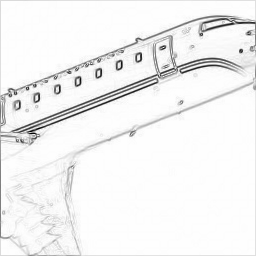
\includegraphics[height=\imgH cm]{Figures/flugzeug_ds_emse.png}};
\node[above=2pt of imgL, anchor=south, font=\scriptsize] {Edge Map (Input)};

% Pfeil 2 cm nach rechts als Anker für die Box
\coordinate (boxAnchor) at ($(imgL.east)+(2cm,0)$);

% === TSD-Hauptbox ===
\node[bigbox, anchor=west,
      minimum width=\boxW cm, minimum height=\boxH cm] (tsdBox) at (boxAnchor) {};
\node[font=\bfseries, anchor=north, text=black]
  at ([yshift=-4pt]tsdBox.north) {TSD};

% --- Interne Funktionsblöcke ---
\node[fun, anchor=north west] (mesh)
  at ([xshift=\padX cm, yshift=-\padY cm] tsdBox.north west)
  {Meshing\\(\texttt{target control points 5$\times$5})};

\node[fun, anchor=north west] (rnd)
  at ([yshift=-0.90 cm] mesh.south west)
  {Random Offsets\\(\texttt{sample noise with $\lambda$})};

\node[fun, anchor=north west] (tps)
  at ([yshift=-0.90 cm] rnd.south west)
  {TPSGridGen\\(\texttt{Fit $\rightarrow$ warp grid})};

\node[fun, anchor=north west] (warp)
  at ([yshift=-0.90 cm] tps.south west)
  {Apply TPS Warp};

% --- Flows in der Box (Labels = Output der jeweiligen Box) ---
\draw[flow] (imgL.east) -- (mesh.west);

\draw[flow] (mesh.south) -- (rnd.north)
  node[flowlabel, above]{CP grid (5×5)};

\draw[flow] (rnd.south) -- (tps.north)
  node[flowlabel, above]{Perturbed CPs};

\draw[flow] (tps.south) -- (warp.north)
  node[flowlabel, above]{Warp grid $[H\times W\times 2]$};

% ==== Mini-Bild 1 (rechts von Meshing) mit REGULÄREM 10x10 Grid ====
\def\thumbW{2}      % Breite Mini-Bild [cm]
\def\thumbDx{1.2}     % Abstand zur Box [cm]

\node[imgframe, anchor=west, inner sep=0pt] (meshImg)
  at ($(mesh.east)+(\thumbDx,0)$)
  {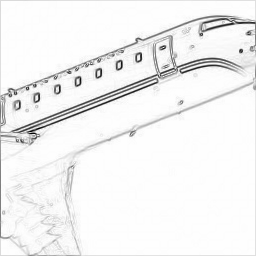
\includegraphics[width=\thumbW cm]{Figures/flugzeug_ds_emse.png}};
\node[above=0pt of meshImg, anchor=south, font=\scriptsize] {CP Grid};

\draw[dashed, line width=0.8pt] (mesh.east) -- (meshImg.west);

% ===== Global: reguläres Grid + Punkte =====
\def\cpCount{5}        % Kontrollpunkte pro Achse
\def\meshLineW{.6pt}    % Linienstärke der Rasterlinien
\def\cpDotR{1.2pt}      % Radius der roten Punkte
\pgfmathsetmacro{\meshStep}{1/(\cpCount-1)} % Schrittweite in [0,1]

% --- Raster + Punkte exakt über dem Bild (REGULÄR) ---
\begin{scope}[
  shift={(meshImg.south west)},
  x={(meshImg.south east)-(meshImg.south west)},
  y={(meshImg.north west)-(meshImg.south west)}
]
  % Rahmen (optional)
  \draw[red, line width=\meshLineW] (0,0) rectangle (1,1);

  % Vertikale Linien
  \foreach \i in {0,...,\numexpr\cpCount-1\relax} {
    \pgfmathsetmacro{\t}{\i*\meshStep}
    \draw[red, line width=\meshLineW] (\t,0) -- (\t,1);
  }
  % Horizontale Linien
  \foreach \j in {0,...,\numexpr\cpCount-1\relax} {
    \pgfmathsetmacro{\u}{\j*\meshStep}
    \draw[red, line width=\meshLineW] (0,\u) -- (1,\u);
  }

  % Punkte an allen Kreuzungen
  \foreach \i in {0,...,\numexpr\cpCount-1\relax} {
    \pgfmathsetmacro{\t}{\i*\meshStep}
    \foreach \j in {0,...,\numexpr\cpCount-1\relax} {
      \pgfmathsetmacro{\u}{\j*\meshStep}
      \fill[red] (\t,\u) circle[radius=\cpDotR];
    }
  }
\end{scope}

% ==== Mini-Bild 2 (rechts von TPSGridGen) mit VERZERRTEM 10x10 Grid ====
\node[imgframe, anchor=west, inner sep=0pt] (tpsImg)
  at ($(tps.east)+(\thumbDx,0)$)
  {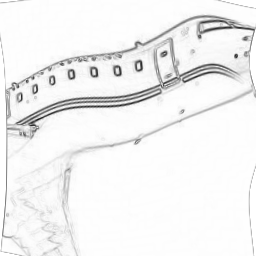
\includegraphics[width=\thumbW cm]{Figures/flugzeug_tsd.png}};
\node[above=0pt of tpsImg, anchor=south, font=\scriptsize] {Warp Grid};

\draw[dashed, line width=0.8pt] (tps.east) -- (tpsImg.west);

% ===== Global: verzerrtes Grid-Parameter =====
\def\lam{0.03}              % max. Offset in Normkoordinaten (2%)
\def\distMode{uniform}      % uniform | normal
\pgfmathtruncatemacro{\N}{\cpCount-1}
\pgfmathsetseed{2025}       % reproduzierbar

% --- Verzerrtes Raster + Punkte exakt über dem Bild ---
\begin{scope}[
  shift={(tpsImg.south west)},
  x={(tpsImg.south east)-(tpsImg.south west)},
  y={(tpsImg.north west)-(tpsImg.south west)}
]
  % 1) Knoten Pij mit Randfixierung + Random Offsets (innen)
  \foreach \i in {0,...,\N} {
    \pgfmathsetmacro{\tx}{\i*\meshStep}
    \foreach \j in {0,...,\N} {
      \pgfmathsetmacro{\ty}{\j*\meshStep}
      % Rand?
      \pgfmathsetmacro{\isEdge}{(\i==0) || (\i==\N) || (\j==0) || (\j==\N)}
      \pgfmathsetmacro{\dx}{0}
      \pgfmathsetmacro{\dy}{0}
      \ifdim \isEdge pt=0pt
        \ifnum\pdfstrcmp{\distMode}{normal}=0
          % Normalverteilung via Box-Muller
          \pgfmathsetmacro{\uone}{max(1e-6,rnd)}
          \pgfmathsetmacro{\utwo}{rnd}
          \pgfmathsetmacro{\gaussA}{sqrt(-2*ln(\uone))*cos(360*\utwo)}
          \pgfmathsetmacro{\uoneb}{max(1e-6,rnd)}
          \pgfmathsetmacro{\utwob}{rnd}
          \pgfmathsetmacro{\gaussB}{sqrt(-2*ln(\uoneb))*sin(360*\utwob)}
          \pgfmathsetmacro{\dx}{\lam*\gaussA}
          \pgfmathsetmacro{\dy}{\lam*\gaussB}
        \else
          % Gleichverteilung in [-lam, +lam]
          \pgfmathsetmacro{\dx}{\lam*(2*rnd-1)}
          \pgfmathsetmacro{\dy}{\lam*(2*rnd-1)}
        \fi
      \fi
      \coordinate (Q\i\j) at ({\tx+\dx},{\ty+\dy});
    }
  }

  % 2) Linien zeichnen (Polylinien)
  % Vertikale Linien (i = const)
  \foreach \i in {0,...,\N} {
    \draw[red, line width=\meshLineW]
      (Q\i0) \foreach \j in {1,...,\N} { -- (Q\i\j) };
  }
  % Horizontale Linien (j = const)
  \foreach \j in {0,...,\N} {
    \draw[red, line width=\meshLineW]
      (Q0\j) \foreach \i in {1,...,\N} { -- (Q\i\j) };
  }

  % 3) Punkte
  \foreach \i in {0,...,\N} {
    \foreach \j in {0,...,\N} {
      \fill[red] (Q\i\j) circle[radius=\cpDotR];
    }
  }
\end{scope}

% Bild rechts bleibt auf gleicher Höhe wie das Input-Bild
\node[imgframe, anchor=west] (imgR)
  at ($(tsdBox.east |- imgL)+(2cm,0)$)
  {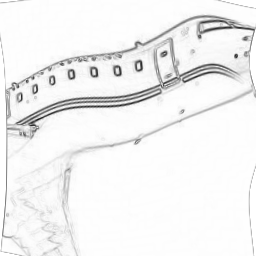
\includegraphics[height=\imgH cm]{Figures/flugzeug_tsd.png}};
\node[above=2pt of imgR, anchor=south, font=\scriptsize] {Deformed Edge Map (Output)};

% Pfeil: erst 3 cm nach rechts, dann schräg direkt zum Bild (kein rechter Winkel)
\draw[flow,shorten >=1pt]
  (warp.east) -- ++(4cm,0) -- (imgR.west);



\end{tikzpicture}
\end{document}
